% This file is iccc.tex.  It contains the formatting instructions for and acts as a template for submissions to ICCC.  It borrows liberally from the AAAI and IJCAI formats and instructions.  It uses the files iccc.sty, iccc.bst and iccc.bib, the first two of which also borrow liberally from the same sources.

\documentclass[letterpaper]{article}
\usepackage{iccc}

\usepackage{graphicx}
\usepackage{times}
\usepackage{helvet}
\usepackage{courier}
\pdfinfo{
	/Title (Anything2vec: generalizing word2vec via the use of meaningful contexts)
	/Subject (Proceedings of ICCC)
	/Author (ICCC)}
% The file iccc.sty is the style file for ICCC proceedings.
%

%\title{Anything2vec: generalizing word2vec via the use of meaningful
%	contexts}
% Add something about its application to trope description - JJ 
%\author{Dan Ventura\\
%Computer Science Department\\
%Brigham Young University\\
%Provo, UT 84602  USA\\
%ventura@cs.byu.edu\\
%}
\setcounter{secnumdepth}{0}

\begin{document} 
	% \maketitle
	\begin{abstract}
		\begin{quote}
			% From the old paper:
			%   Word2vec has been a very successful algorithm that is able to give a
			% semantic representation to words on a corpus based in the context
			% they appear. In this paper we will try to extend this concept to
			% other {\em unordered} contexts. We will try to define this context
			% for movie (and TV) tropes.
			In this paper we present a generalized approach to extend the use of word2vec for non-traditional NLP (Natural Language Processing). In order to exemplify the idea, we use tvtropes dataset (trope names and film names only) to create a text corpus in order to give contextual information to any piece of data.
		\end{quote}
	\end{abstract}
	
	% From the old paper:
	% What are tropes and why we are interested
	
	% We need to find an embedding for tropes that allows us to do trope arithmetic and also process them, and movies in which they are used, in an uniform way.
	
	% We propose trope2vec
	
	% We analyse how it allows to explore the trope space and find
	% similarities between them.
	
	\section{Introduction}
	
	% Some help from: https://www.nature.com/scitable/topicpage/scientific-papers-13815490/
	
	% First, provide some context to orient those readers who are less familiar with your topic and to establish the importance of your work.

    % With growing diversity in personal food preference and regional cuisine style, personalized information systems that can transform a recipe into any selected regional cuisine style that a user might prefer would help food companies and professional chefs create new recipes.
    
    
 
    When we want to work with vector representations of words, word2vec is one of the most used algorithms since its appearance \cite{mikolov2013}.
    The vector obtained for each word has the ability to save memory of its environment. This vector is called embedding vector.
    Another interesting feature of embeddings vectors is that it is possible to perform concept arithmetic. For example, it would be possible to subtract and add vectors so that we obtain another vector resulting from the operation: Paris - France + Italy = Rome. However, in order to apply this algorithm, it is necessary to have a sufficiently large corpus written in natural language. Some examples of these frequently used corpus are Wikipedia or Google News dumps, usually greather than one GB of plain text. \\
    
    But, it would be possible to apply word2vec to non natural language corpus? With this work we want to demonstrate that it is possible to obtain embeddings vectors using word2vec of an artificially created corpus. To demonstrate this idea we will use data from films and tropes obtained from tvtropes.org website. Tv Tropes is a collaborative website created in 2004 to share information about tips, narrative or cinematographic techniques used in creative works such as movies, tv series or books. Each film, TV series or other
    fiction element usually includes a description and a list of associated
    tropes. Tropes pages usually contains a description followed by a list
    of films or a narrative resource that uses this trope.\\
    
	% Second, state the need for your work, as an opposition between what the scientific community currently has and what it wants.
	
	Obtaining a vector representation of concepts is an old problem that can be solved in different ways. Some of these solutions use only word coding without considering the context. This type of representation has a more limited use. Other works like \cite{kazama2018} have shown that it is
	possible to use word2vec to obtain vectors from non-NLP information
	sources. Our approach is based on the use of the fundamental elements
	of information (in our case the tropes) to generate an artificial
	narrative or corpus that can give a similar meaning to the concepts
	that they would have in a text written by humans. This artificially
	created text should represent the relationships between entities in
	the same way that a human would relate them in a descriptive text
	about these entities. If the artificial corpus is correctly
	constructed, it should produce some embedding vectors with the
	capacity to offer us a correct arithmetic of concepts. 
	
	We want the word representation to have the following characteristics: 
	
	\begin{itemize}

	\item That includes the context of the trope
	\item relatively compact
	\item capable of doing arithmetic
	\item uniform for tropes and movies.
		
    \end{itemize}
	   
    % I need help to write this part   
	   
	% Third, indicate what you have done in an effort to address the need (this is the task).

    In order to solve the problem, we have downloaded films data from word2vec. Then we have extracted a subset of films whose number of tropes is less than a certain thresold. From this subset of films and tropes, we have built an artificial corpus on which to apply the word2vec algorithm and generate embeddings. To evaluate that the subset of tropes is representative, we have verified that 92\% of the subset are among the most frequently used tropes. With the obtained vectors we have generated a classification to verify correspondence between embeddings and real films-tropes relationships. From the vectors that represent the tropes we have created a vector for the film. As a result, we have verified that the artificially generated corpus fulfills the desired objective. Obtained graphic representation shows that obtained clusters are correlated with real relationships observed between tropes and between tropes and films.\\
 
 % How we want to solve that problem: we think that an adaptation of word2vec should be possible
 % This is what you say above - JJ	
		% How we do it:
	% * Methodology for creating the context of every trope
	% * Methodology for representing movies using trope vector
	% * How we evaluate the goodness of the set of movies/tropes chosen.
	
	% Our results
	% * Clustering
	% * Graph representation
	% * Movie representation
	% * Example of synthetic movie generation.
	
	
	% Finally, preview the remainder of the paper to mentally prepare readers for its structure, in the object of the document.

	The rest of the paper is organized as follows. Next we present the
	state of the art in using embedding for problems other than language
	processing, as well as an overview of the use of tropes for narrative
	generation. The methodology is presented next in Section
	\ref{sec:met}, with results presented in Section \ref{sec:res}
	followed by the conclusion that closes the paper.
	
	
	\section{State of the art}
	
	Unlike systems such as MovieLens \cite{10.1145/2827872}, which focus
	on recommendation, our ultimate
	interest in representing movie tropes lies in the possibility of
	generating narratives \cite{10.5555/931357} that are optimal from some point of view (mainly
	coherence) from a set of tropes. Out of all the possible methods to
	generate narratives \cite{van2019narrative} this is one that has
	probably been explored the least; Sullivan et
	al. \cite{10.1145/3235765.3235819} used tropes in the tarot deck to
	generate narratives via combinations, but other than that, in general
	the presence of tropes has been used more for evaluation of generated
	narratives \cite{gervas2012story} that as part of the generation
	itself; in general, tropes are understood as constraints for
	characters or plots \cite{Thompson18NarrativeEvents}, but, of course,
	there are many kind of tropes and some of them can be converted
	directly into plots; for instance, {\sf AgeStereotypicalFood} informs
	of the fact that eating or talking about food will be introduced into
	the narrative.
	
	This work has been inspired by other that have used
	word2vec-like embeddings for purposes that are totally
	unrelated to natural language; a good survey is presented in
	\cite{nonnlp19}. In general, creating embeddings out of data
	is done with several purposes: reducing dimensionality, but
	also trying to create a data representation with semantics; as
	a side effect, this data representation will enable ``content
	arithmetics''. In our previous work
	\cite{doi:10.1111/exsy.12525} we used a direct representation
	of tropes; every dimension in a vector represented a trope,
	once less frequent ones had been excluded. However, this left
	out many possibly meaningful tropes, and still the size of the
	vectors was huge, representing its own challenge when using
	them in a deep learning algorithm.
	
	This was one of the intentions of Kazama et al. in
	\cite{kazama2018}, which is actually the paper that inspired
	our work. The content they wanted to represent was the concept
	of ``regional cuisine'', so that a regional cuisine embedding
	could be added or substracted from the embedding of a dish to
	create a new, equivalent one in that new regional
	environment. The kind of data they were working with is
	similar to the one we use in this paper: dish ingredients. As
	in our case, there's no natural order in the ingredients, but
	unlike our case, the amount of ingredients that are used in a
	dish are really limited, at least if you exclude
	seasoning. But they achieved their objective: being able to do
	recipe arithmetics, but also create meaningful maps of food
	that can be used in deep learning or any other environment.
	
	Most other applications are similar, in a way, to this one,
	and most of them are also recent. There was a publication in
	the Twitter engineering blog \cite{twitter:embeddings},
	apparently pointing to their use studying the social networks
	of users. Initial work was done by Grbovic et al. applied it to product recommendation
	\cite{Grbovic2015}, Vasile et al. applied it to product
	recommendation systems \cite{vasile2016} while McAuley et
	al. \cite{DBLP:journals/corr/McAuleyPL15} used embedding
	arithmetics to find complementary products to others that had
	been already purchased; these articles were
	probably ones of the first to use this kind of
	representation.
	
	Word embeddings to create clustering, however, go back at
	least to Kohonen's work in the 90s
	\cite{kohonen1997exploration}, which tried to create
	embeddings by assigning a word a vector created from averaging
	randomly created vectors initially assigned to its neighboring
	vectors. This work was extended to ant clustering algorithms
	to create word clusterings by Ramos et
	al. \cite{DBLP:journals/corr/abs-cs-0412075}.
	
	The fact that the variety of data embeddings have been applied
	to, as well as the kind of applications created with is so
	wide, has encouraged us to apply it to the study of movies via
	their tropes, as well as its eventual optimization.
	
	\section{Methodology}
	\label{sec:met}
	
	In order to evaluate the goodness of artificial corpus for embedding vectors generation, two different approaches have been analyzed:
	\begin{enumerate}
		\item For the first version we have generated the corpus through tropes permutations and adding film name in each phrase. In order to simplify the process of creating and verifying accuracy we have selected films with a maximun number of tropes per film. Table \ref{tab:corpusSize} shows how the maximum number of tropes affects the size of the corpus.
		
        \item For the second method, we have created the corpus through relationships reinforcement between tropes and films as if it were a relational database. In order to compare both approaches we have selected same films for both methods.
	 \end{enumerate}
 
    \subsection{Construction of artificial corpus: trope permutation approach}
    
    This approach uses tropes permutation as a method of creating corpus phrases. Next to the selection of permuted tropes the name of the film is added in order to connect the film with their tropes. In this approach the relationship between film and their tropes is lighter, since film name will be next to nine other tropes. The relationship between the different tropes is also not reinforced by any criteria, we simply sort group of tropes randomly. Before deciding which maximum number of tropes per film and the size of phrase (ngram) is most appropriate, we have performed different tests. Table \ref{tab:corpusSize} shows different values for MAX\_TROPE and NGRAM\_SIZE. After different tests we have decided to take the values 15 and 9 respectively to create corpus. We take this
    initial limit since we will generate all the variations
    without repetitions of 15 elements taken in groups of 9
    elements. This method can give us enough size corpus to train
    the model using word2vec algorithm. This method consists of the following steps:
	
	\begin{enumerate}
		\item Getting film data from tvtropes.org and their associated tropes
		\item Select films with number of tropes less than a certain thresold
		\item Create phrases from permutations of the tropes associated with each movie and including film name in each phrase
		\item Build word2vec model. After that we will obtain an embedding vector for each film and trope
		\item Generate accuracy check list 
		\item Check model accuracy using generated check list
		\item Visualize tropes vector space in order to detect clusters and possible data organization.
    \end{enumerate}

	% Main idea here is that the artificial corpus will represent the true as much as possible. ¿how we can achieve that?
	% We need a parameter that let us reinforce more real relationships between elements that are stronger. For example, in case of films,
	% we can use a value of film popularity to write more times in corpus information about a blockbuster film. We have to do the same with 
	% es like tropes. More relevant tropes will be them who appear more times in films, so these tropes have to appear more times in 
	% corpus. Ideal situation will be that artificial corpus emulate real conextions faithfully.\\
	% Let's use imdb blockbuster films sort by votes. Votes will be the number to reinforce more in corpus films that have more votes.	 
	% we can apply an incremental approach to do that, creating verification check lists to see if certain part of the corpus fits reality. 
	% for next paper version

    \subsubsection{Getting film data}
		
	\begin{table}[t]
		\centering
		\begin{tabular}{|p{0.24\linewidth}|p{0.18\linewidth}|p{0.18\linewidth}|p{0.18\linewidth}|}
			\hline
			\textbf{(Max\_Tropes, Ngram\_Size)}& \textbf{(16,9)} & \textbf{(15, 9)} & \textbf{(12,7)}\\
			\hline
			\hline
			Tropes Subset Size&8125&7383& 5500\\
			\hline
			Film Subset Size&2686&2380& 1674\\
			\hline
			Corpus File Size (MB)&747&264& 32\\
			\hline
			Word2vec Model file Size(MB)&5.6&4.9&4.9\\
			\hline
			Vocab Size& 7078 & 6173 & 4653\\
			\hline
			Words in train file& 48893099 &17386514&2056372\\
			\hline

		\end{tabular}
		\caption{Characteristics of different corpus sizes and word2vec models created by varying MAX\_TROPES and NGRAM\_SIZE (word2vec argument min-count = 5, MIN\_TROPES = 2)}
		\label{tab:corpusSize}
	\end{table}
	
	After downloading films and tropes data from tvtropes.org (on date 13th December 2019) and processing the obtained information, we get 12360 movies and 26742 (25405 after remove repeated) tropes. The film with higher number of tropes has 1028 tropes and the film with minimum number of tropes has 0 tropes.
	
	\subsubsection{Select films and tropes}
	From all these data we must filter repeated elements and get only those films that have between 15 and 2 tropes and their associated tropes. After selecting this group of films we get 2380 films and 7383 tropes.
	Figure \ref{fig:tropesdistributionasociatedtofilms} shows the distribution of films by number of tropes and the cumulative total of tropes. Here we can see how for a value of 250 in the maximum number of tropes in a film 98.4\% of the tropes are covered. In order to check if our subset of tropes is relevant, we sort the tropes by frequency of occurrence. We verify that in our subset is 99.2\% of the most popular tropes, so we can consider it a representative subset. In order to obtain the most popular tropes we obtain all  film-trope pairs, a total of 599341 different pairs. Counting number of times that each trope appears in film-trope pairs list, we will obtain use frequency of each trope. 
	
	\begin{figure}
		\centering
		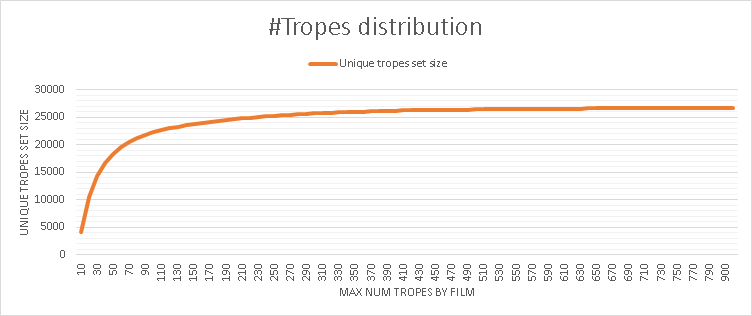
\includegraphics[width=1\linewidth]{../images/tropes_distribution_chart.png}
		\caption{Accumulative distribution of tropes associated to films}
		\label{fig:tropesdistributionasociatedtofilms}
	\end{figure}
	
	\subsubsection{Create corpus by tropes permutation}
	Next step consist of creating an artificial corpus through the permutation of sets of M values taken from N in N. M corresponds to film number of tropes  (MAX\_TROPES) and N with the size of the phrase or NGRAM-SIZE. table \ref{tab:corpusSize} shows different sizes of NGRAM\_SIZE and MAX\_TROPES. We decided to use the values of 15 and 9 respectively since it offers us a corpus size that we consider may be suitable for training. Within each sentence, we include the name of the film by way of creating the relationship between both, films and their tropes. 
	For movies with less than 9 tropes we simply include all of them along with the name of the movie. Finally each sentence is randomly sorted.
	
	\subsubsection{Build word2vec model}
	
	The word2vec algorithm is applied to the generated corpus. For this we use the package \cite{git-hub-word2vec} developed by the creators of the article \cite{mikolov2013}. In model creation process we use bag-of-words algorithm, a 200 dimensions vector of size, a window of size 5 and a min-count of 1 (words that are repeated less than once are eliminated) as main parameters.
	
	%       % This kind of thing does not belong in a paper 
	%     Following line represent word2vec train parameters:\\
	% \begin{verbatim}
	% /word2vec 
	% -train ngrams_15_taken_9.txt 
	% -output ngrams_15_taken_9.bin 
	% -cbow 1 -size 200 -window 8 
	% -negative 25 -hs 0 
	% -sample 1e-4 -threads 20 
	% -binary 1 -iter 15
	% \end{verbatim}
	
	% There's no need to say what to do; focus on the results and the
	% methodology. Mechanical steps can be explained in the repository.
	
	\subsubsection{Generate accuracy check list}
	Creating the accuracy checklist is one of the most creative parts of the methodology. To obtain it we have first observed the checklists contained in the package \cite{git-hub-word2vec}. Table \ref{tab:phrases-check-accuracy} shows some lines of this accuracy checklist. 
	In selected examples, we can verify that univocal pairs are associated. For example in line	Boston Boston\_Globe Chicago Chicago\_Tribune, we can check that 
	Boston\_Globe is one of the main newspapers of Boston city, in the same way that Chicago\_Tribune is one of the main newspapers in Chicago city. Our checklist must also contain univocal relationships. To do this, we select from each film its most popular trope. So we will have, that the relationship will be:
	
	\begin{verbatim}
	<film1> <top-trope1> 
	<film2> <top-trope2>
	\end{verbatim}
	
	In this relationship there is only one top trope for each movie and it would be possible to univocally make reference to it from the movie. In our case it is possible that this top trope is repeated for different films but it will always be the same. Something similar can happen with a very popular newspaper that is based in different cities and it has not a name adapted for each city. Another option may be to create a trope name adapted to the film, as with certain newspapers that adapt their name to the city, as would be the case with The New York Sun or Baltimore Sun. 
	\begin{verbatim}
	<film1> <top-trope1-film1> 
	<film2> <top-trope2-film2>
	\end{verbatim}
	
	This second technique of creating the relationships between films and tropes, making the name of the trope unique for each film, will be used in the second method of corpus creation. Finally, we take a group of movies randomly and associate their top trope. Next, we take first pair (movie, top-trope) and the other selected pairs and we repeat this process with all the films and their associated top tropes. We will use the same accuracy checklist for the two proposed corpus creation methods.   

	\begin{table*}[ht]
		\centering
		\begin{tabular}{|p{0.65\linewidth}|p{0.35\linewidth}|}
			\hline
			Phrases examples & Words examples\\
			\hline	  
			\hline
			: newspapers\\
			\hline
			Albuquerque Albuquerque\_Journal Baltimore Baltimore\_Sun & he she his her\\
			Albuquerque Albuquerque\_Journal Boston Boston\_Globe & he she husband wife\\
			Albuquerque Albuquerque\_Journal Cincinnati Cincinnati\_Enquirer & he she king queen\\
			Albuquerque Albuquerque\_Journal Cleveland Cleveland\_Plain\_Dealer & he she man woman\\
			\hline
			Baltimore Baltimore\_Sun Boston Boston\_Globe& his her husband wife\\
			Baltimore Baltimore\_Sun Cincinnati Cincinnati\_Enquirer & his her king queen\\
			Baltimore Baltimore\_Sun Cleveland Cleveland\_Plain\_Dealer & his her man woman\\
			Baltimore Baltimore\_Sun Charleston Charleston\_Gazette & his her nephew niece\\
			\hline
			Boston Boston\_Globe Cincinnati Cincinnati\_Enquirer & husband wife king queen	\\
			Boston Boston\_Globe Cleveland Cleveland\_Plain\_Dealer & husband wife man woman\\
			Boston Boston\_Globe Charleston Charleston\_Gazette & husband wife nephew niece\\
			Boston Boston\_Globe Chicago Chicago\_Tribune & husband wife policeman policewoman\\
			
			\hline
		\end{tabular}
		\caption{Word2vec phrases to check model accuracy}
		\label{tab:phrases-check-accuracy}
	\end{table*}
	
	\subsubsection{Check model accuracy}
	In order to check the quality of generated embedding vectors, we use the checklist created in the previous step and the program compute-accuracy from \cite{git-hub-word2vec}. This program returns the number of tuples that have generated the expected value through the model. In our case, how many times the correct top trope has been found given a movie, a top trope and a second movie.
	
	\subsubsection{Visualize tropes vector space}
	In order to visualize tropes vector space we have analyzed the different generated clusters using a modified version of the demo-classes.sh script from \cite{git-hub-word2vec}. 
	We have independently visualized some of these groups in a two-dimensional space using the cluster-visualization.py script that makes use of the gensim, matplotlib libraries and the Principal Component Analysis algorithm from sklearn python library. We have also verified by taking some clusters that the elements included in a grouping are strongly connected on the tvtropes.org website.
	
	\subsection{Construction of artificial corpus: relationships reinforcement approach}
	For corpus construction based on relationship reinforcement approach method, we follow the same methodology as the previous method but modifying step 3.
	
	
	% Main idea here is that the artificial corpus will represent the true as much as possible. ¿how we can achieve that?
	% We need a parameter that let us reinforce more real relationships between elements that are stronger. For example, in case of films,
	% we can use a value of film popularity to write more times in corpus information about a blockbuster film. We have to do the same with 
	% es like tropes. More relevant tropes will be them who appear more times in films, so these tropes have to appear more times in 
	% corpus. Ideal situation will be that artificial corpus emulate real conextions faithfully.\\
	% Let's use imdb blockbuster films sort by votes. Votes will be the number to reinforce more in corpus films that have more votes.	 
	% we can apply an incremental approach to do that, creating verification check lists to see if certain part of the corpus fits reality. 
	% for next paper version
	
	\subsubsection{Create corpus by relationships reinforcement}
	
	
	

	\begin{table}[t]
		\centering
		\begin{tabular}{|p{0.24\linewidth}|p{0.18\linewidth}|p{0.18\linewidth}|p{0.18\linewidth}|}
			\hline
			\textbf{(Max\_Tropes, Ngram\_Size, Min Count)}& \textbf{(15, 9, 1)} & \textbf{(15,9, 3)} & \textbf{(15, 9, 5)}\\
			\hline
			\hline
			Tropes with vector&7383  & 6196 & 6172 \\
			\hline
			Tropes without vector& 0 & 1187 & 1211 \\
			\hline
			Total tropes&7383&7383&7383\\
			\hline
		    Vocab Size& 7384 & 6197 & 6173 \\
			\hline
			Words in train file& 17387907 & 17386591 & 17386514 \\
			\hline 
			
		\end{tabular}
		\caption{Characteristics of different word2vec models created by varying the MIN\_COUNT argument}
		\label{tab:variations-with-min-count-argument-15-9}
	\end{table}	
	

	

	
	\begin{table*}[ht]
		\centering
		\begin{tabular}{|p{0.1\linewidth}|p{0.1\linewidth}|p{0.1\linewidth}|p{0.1\linewidth}|p{0.1\linewidth}|p{0.1\linewidth}|p{0.1\linewidth}|}
			\hline
			\textbf{Num Clusters}& \textbf{500} & \textbf{250} & \textbf{125} & \textbf{64} & \textbf{32} & \textbf{8}\\
			\hline
			\hline
			Vocab Size& 7384 & 7384 & 7384 & 7384 & 7384 & 7384\\
			\hline
			Words in train file& 17387907 & 17387907 & 17387907 & 17387907 & 17387907 & 17387907\\
			\hline
			
		\end{tabular}
		\caption{k-means cluster generation for tropes vectors.Max\_Tropes=15, Ngram\_Size=9, MinCount=1}
		\label{tab:k-means-clusters}
	\end{table*}	
	
	
	
	\section{Results}
	\label{sec:res}
	
		\begin{figure}
		\centering
		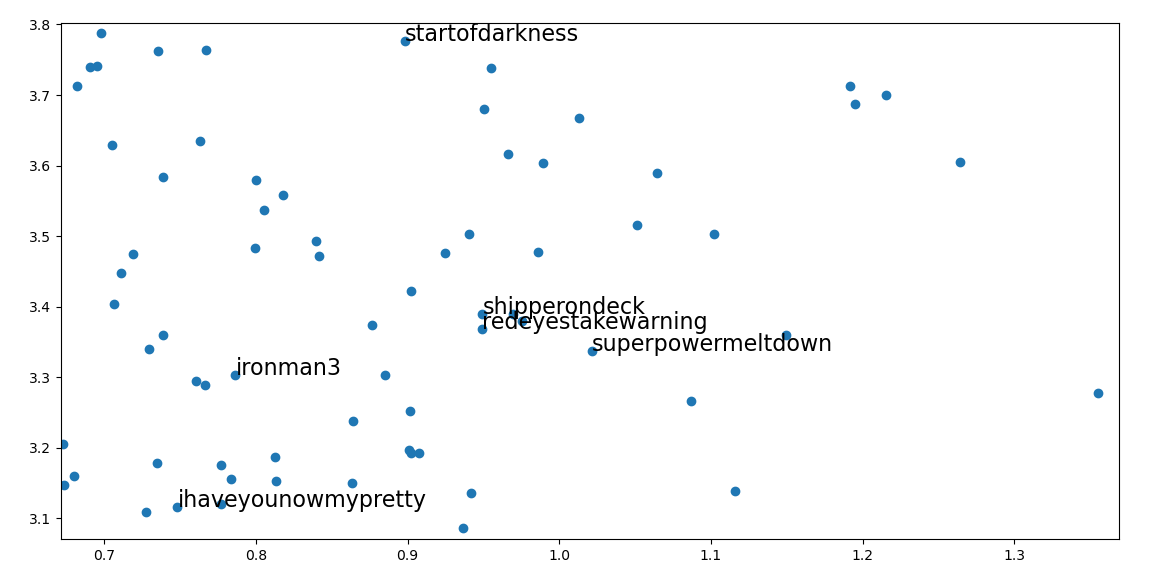
\includegraphics[width=1\linewidth]{../images/cluster-36-visualization-new-corpus-v3-1024-ironman3-font-16-zoom-in.png}
		\caption{Cluster visualization zoom in}
		\label{fig:cluster-visualization-zoom-in}
	\end{figure}
	
	
	\begin{figure}
		\centering
		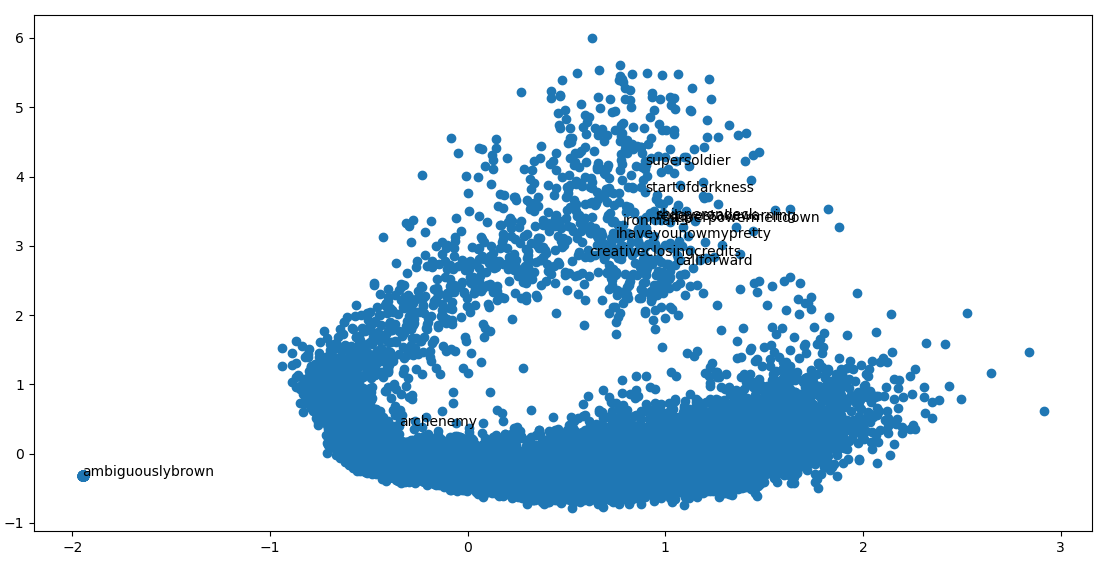
\includegraphics[width=1\linewidth]{../images/cluster-36-visualization-new-corpus-v3-1024-ironman3-zoom-out.png}
		\caption{Cluster visualization zoom out}
		\label{fig:cluster-visualization-zoom-out}
	\end{figure}
	
	
	
	\section{Conclusions, discussion and future work}
	 
	From the obtained results we can conclude that the fact of creating an artificial corpus improves the accuracy of the embedding vectors generated in relation to a natural language  corpus. The fact of being able to build the custom corpus allows us to avoid rhetorical elements derived from the use of natural language. In this way we can put the focus on the relationships between the entities and always put together those words that are related. We avoid so words that do not have a strong relationship appear close. 
	We have found two main difficulties when implementing this methodology:
	\begin{itemize}
	\item The first has been to find a metric that allows us to reinforce more important concepts. 
	\item Second one, has been to obtain a metric that allows us to evaluate the results.
    \end{itemize}
	It will be necessary to find these metrics in each problem where you want to apply this methodology
	
	Future work should focus on finding new ways to measure the accuracy of the results. In many cases finding relationships between entities is trivial when it comes to natural language. Clear examples of this can be the capitals of countries or find the feminine of some term. However, trying to achieve the same in areas where we are not very familiar can be much more complicated. Finding metrics that allow us to evaluate the accuracy of the model without the need to have a very deep knowledge of the work area would be an interesting future line of work. Another question worthy of being analyzed in future works, consists in finding characteristics in the real system that serve to reinforce with greater intensity those stronger relationships. In the dataset used we have used the popularity of films and tropes as a means of reinforcing more intensely the relationships between films and popular tropes. Better markers will allow the models to more accurately represent the relationships between the entities of the real system.
	
	
	% It is possible to create artificial corpus better than natural ones?
	
	% find other ways to build accuracy checklists 
	% Popular films will appear more times in corpus. This idea can be used to build the artificial corpus in future works.
	% Check if embedding vectors clusters can be used to obtain better accuracy check lists 
	\section{Acknowledgments}
	
	\bibliographystyle{iccc}
	\bibliography{iccc}
	
\end{document}
